\scanpage{150}
Azumaya rang $4$ \quad (III) \hfill Avril $86$

\figure{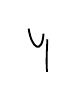
\begin{tikzpicture}[x=0.18cm,y=0.18cm]
\draw[line width=.7pt] (0,2.7) .. controls (.2,1.3) and (.95,.85) .. (1.05,2.35);
\draw[line width=.65pt] (1.32,1.95) .. controls (1.29,1.15) and (1.23,.35) .. (1.3,-.35);
\end{tikzpicture}}
\uline{Digression} sur les produits tensoriels d'espaces affines à involution.

``La donnée, sur un $k$-module $H$ muni d'un élément $1_H$ (``unité'') \inserted{tel que $\lambda\longmapsto\lambda1$ soit injectif de $k$ ds $H$}, d'une \deleted{involution} \inserted{appl. lin.} $x\longrightarrow x'$ qui a) fixe $1_H$ et b) \unsure{induiste|induise|induit} sur $H/k1$ la symétrie, i.e. $x'\equiv-x\bmod k.1$, i.e. $x+x'\in k.1$, équivaut à la donnée d'une forme linéaire $T:H\longrightarrow k$ telle que $T(1_{\unsure{H|.}})=2$, et on aura
% slanted
\margin{i.e. on a une ``coaugmentation'' $k\longrightarrow H$}
\[
 x'=T(x).1-x
\]
\margin{alors $x\longrightarrow x'$ est involutive}

Dualement, \deleted{la donnée} quand on a un $k$-module $E$ et une augmentation
\[
 E\xrightarrow{\varepsilon} k
\]
surjective (ce qui revient à se donner un espace affine \inserted{$A=\varepsilon^{-1}(1)$ sur $k$}, dont le \deleted{\unsure{mo}}module des translations sera $A^0=\operatorname{Ker}(\varepsilon)$), \deleted{revient à se donner un} \inserted{la donnée d'une} involution de $E$ compatible avec $\varepsilon$ (avec id. dans $k$) et induisant sur $A^0=\operatorname{Ker}\varepsilon$ la symétrie $x\longrightarrow-x$, revient à se donner un élément
\[
 t\in E\qquad\text{avec}\qquad\varepsilon(t)=2,
\]
l'involution sera alors
\[
 x\longrightarrow\varepsilon(x)t-x
\]
et $t$ sera fixe. Se donner un espace affine $A$ sur $k$, muni d'un \deleted{\unsure{endo}} \unsure{endom.|involution} qui induise $-\mathrm{id}$ sur le module des translations, revient à se donner un tel syst. (et \deleted{\unsure{l'endom.}} \unsure{autm|élément} est alors involutif).
% archive sheet number: 149

